\subsection{Real-world data for simulation}

To do our numerical simulations, we will consider the thermal conducitivty, density and heat capacity to be constants, we divide by $\rho c_p$ in \eqref{eq:heat} to get 
\begin{equation*}
    \theta_t - \alpha \nabla \cdot (\nabla \theta) = 0 \quad \text{in $\Omega \times (0,T)$ }
\end{equation*}
Here $\alpha = \frac{k}{\rho c_p}$ is the Thermal diffusivity. Now this is a simplifiction of the model, as more realistically the heat conductivity is temperature dependent i.e. $k = k(\theta)$ and the heat capacity depends on heat conductivity $c_p = c_p(k)$. We set the parameters as shown in Table \ref{tab:chosenParam} when doing our simulation of the heat evolution in our multiphase steel, values are similar to \cite{DPSteel}. 
\begin{table}[h]
    \centering
    \caption{Parameters used for numerical simulation of the rolling of steel process.}
    \begin{tabular}{@{}lr@{}} \toprule
    $\text{Parameter}$ & $\text{SI-unit}$ \\
    \midrule
       $k$& $\SI{50.2}{\joule\per\metre\per\second\per\kelvin}$ \\
        $c_p$ & $\SI{509.6}{\joule\per\kilogram\per\kelvin}$ \\
        $\rho$ & $\SI{7850}{\kilogram\per\metre\cubed}$ \\
        $\theta_w$ & $\SI{20}{\celsius}$ \\
        $\theta_d$ & $\SI{700}{\celsius}$ \\
        $\theta_0$ & $\SI{1200}{\celsius}$ \\ \bottomrule
    \end{tabular}
    \label{tab:chosenParam}
\end{table}
Here $\theta_0$ represent the initial temperature of the steel slab shown in \ref{fig:steel_slab}, while $\theta_w$ is the temperature of the applied coolant. To have a realistic size of the slab one might choose $\Omega = (0,7.5)\times(0,0.7) \text{cm}^2$

To test our solution procedure of the state system, we use the parameters of Table \ref{tab:chosenParam} togheter with various choices of $u$. We then verify that the solutions behave as expected. One such example is shown in \ref{fig:state_simulations}. The simulations were produced using a finite element method (FEM) as implemented in the Python package \verb|FEniCS|~\cite{fenics}. For the first choice we sat $u(t) = 1$ we observe that in Figure \ref{fig:state_simulations_a} the temperature is steadily decreasing, as one would expect when continously applying a coolant to the steel. Other runs with different choices of $u$ also behaved as one would expect. Thus, we conclude that the parameters we have chosen are reasonable, and that the model and the simulation of the state system both perform well.
\begin{figure}
    \makebox[\linewidth]{
        \centering
    \begin{subfigure}[t]{3.5in}
        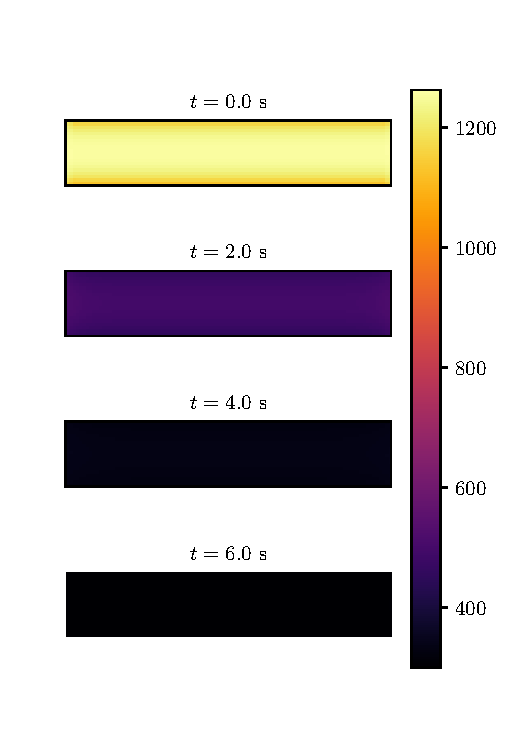
\includegraphics{figures/uniform_u_state.pdf}
        \caption{The state $\theta$ as solved at different time points.}
        \label{fig:state_simulations_a}
    \end{subfigure}
    ~
    \begin{subfigure}[t]{3.5in}
        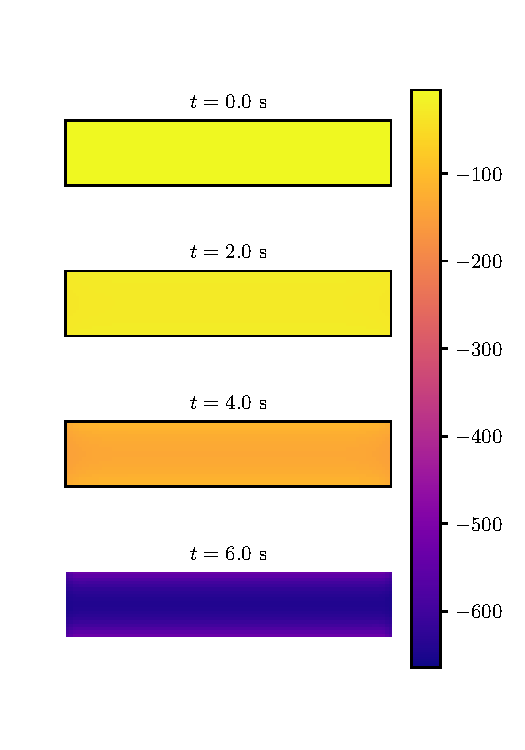
\includegraphics{figures/uniform_u_adjoint.pdf}
        \caption{The adjoint $p$ as solved at different time points.}
        \label{fig:state_simulations_b}
    \end{subfigure}
    }
    \caption{Simulations using the parameters given in Table \ref{tab:chosenParam}. In addition, the initial temperature of the steel was set to \SI{1300}{\celsius}. A constant control $u(t) = 1$ was used.}
    \label{fig:state_simulations}
\end{figure}
